\section{Abfahrtspläne}

Im Gegensatz zur klassischen Planung von Fahrplänen, arbeiten wir nicht mit festgelegten Ankunfts- und Durchfahrtzeiten an den einzelnen Stationen. Stattdessen legen wir lediglich die Abfahrtszeiten an den Startstationen fest und bestimmen dann die Ankunftszeiten an den Zwischenstationen und der Endstation durch Simulation. Daher wird zur Abgrenzung von dem Begriff Fahrplan hier der Begriff \emph{Abfahrtsplan} eingeführt. Im Gegensatz zu einem Fahrplan enthält ein Abfahrtsplan lediglich folgende Informationen:
\begin{itemize}
    \item Die Zuggattung (im Folgenden ''Zugtyp'' genannt)
    \item Die Abfahrtszeiten an der Starthaltestelle
    \item Eine Liste der Zwischenhaltestellen und die Endhaltestelle, jedoch keine Ankunfts- oder Abfahrtzeiten
\end{itemize}
 Wie bereits in den Anforderungen angedeutet, werden drei verschiedene Arten von Abfahrtsplänen benötigt. Solche, die zeitlich regelmäßige Zugfahrten beschreiben (regelmäßige Abfahrtspläne), solche, die Zugfahrten mit zufälligen Abfahrtszeiten beschreiben (zufällige Abfahrtspläne) und solche, deren Abfahrtzeiten sich nach einem historischen Kohlebedarf richten (bedarfsorientierte Abfahrtspläne). Jeder Abfahrtsplan hat einen Startzeitpunkt $t_s \in \mathbb{N}$ und einen Endzeitpunkt $t_e \in \mathbb{N}$. Da hier eine diskrete Zeitachse betrachtet wird, handelt es sich bei den Zeitpunkten um natürliche Zahlen. Der Zeitpunkt $t_s$ beschreibt den Zeitpunkt in der Simulation, wenn der Abfahrtsplan aktiv wird, $t_e$ beschreibt den Zeitpunkt, wenn der Abfahrtsplan deaktiviert wird. Für jeden Abfahrtszeitpunkt eines Zuges $t_a$ gilt also $t_s\leq t_a \leq t_e$. Die Details der drei Varianten werden im Folgenden erklärt.

\paragraph*{Regelmäßige Abfahrtspläne}

Der regelmäßige Abfahrtsplan beschreibt die Abfahrt von Zügen in regelmäßigen zeitlichen Abständen und dient der Modellierung von klassischem fahrplan-basiertem Verhalten. Er hat eine Periode $p\in\mathbb{N}$ in Sekunden, welche die Größe des zeitlichen Abstandes angibt. Ein regelmäßiger Abfahrtsplan lässt somit Züge zu den Zeitpunkten $t_a=t_s+np$ mit $n\in\mathbb{N}$, unter der Einschränkung $t_a\leq t_e$, abfahren.

\paragraph*{Zufällige Abfahrtspläne}

Der zufällige Abfahrtsplan beschreibt die Abfahrt von Zügen in zufälligen zeitlichen Abständen. Er dient damit der Modellierung von Zügen, die unplanmäßig oder unvorhergesehen kurzfristig fahren. Dieser Abfahrtsplan hat eine Wahrscheinlichkeitsverteilung P, die angibt, mit welcher Wahrscheinlichkeit zu jedem diskreten Zeitpunkt der Simulation ein Zug erzeugt wird. P folgt einer Gleichverteilung. Die Wahrscheinlichkeit für eine Abfahrt ist also zu jedem Zeitpunkt gleich. Allerdings kann maximal ein Zug zu einem bestimmten Zeitpunkt abfahren.

\paragraph*{Bedarfsorientierte Abfahrtspläne}

Der bedarfsorientierte Abfahrtsplan beschreibt die Abfahrt von Zügen in zeitlichen Abständen, die sich nach einem historischen Kohlebedarf richten. Er dient damit der Modellierung von Kohlezügen. Dieser Abfahrtsplan hat eine Kohlebedarfsfunktion $k:\mathbb{N}\to\mathbb{R}$, die angibt, wie viel Kohle zu einem Zeitpunkt $t$ benötigt wird. Sie ergibt sich aus den historischen Kohlebedarfsdaten. Weiterhin sind der Zeitpunkt $t_0 \in \mathbb{N}$, an welchem die historischen Daten beginnen und die Zeitspanne $t_r \in \mathbb{N}$, welche die zeitliche Auflösung der Daten angibt, definiert. Außerdem ist $c\in\mathbb{R}$ die Menge an Kohle, die ein Kohlezug transportieren kann.  Sowohl $t_0$, als auch $t_r$ und $c$ sind konstant und ergeben sich aus domänenspezifischen Vorgaben. Zur Berechnung der Abfahrtszeiten wird zunächst die Funktion $a: \mathbb{N} \to \mathbb{R}$ aufgestellt, die den akkumulierten Kohlebedarf zum Zeitpunkt $t$ berechnet (siehe \autoref{eq:kohle-accu}). Dabei ist $n\in\mathbb{N}$ die Anzahl der Datenpunkte.

\begin{equation}
    a(t)=\sum_{i=0}^{\left(\frac{t-t_0}{t_r}\right)} k(t_ri+t_0)\label{eq:kohle-accu}
\end{equation}

Der Abfahrtsplan soll nun stets dann Züge abfahren lassen, wenn die Menge an Kohle, die transportiert werden muss, die Menge erreicht, die ein Zug transportieren kann. Die transportierte Menge wird dann von der bisher akkumulierten Menge abgezogen. \autoref{eq:kohle-fmod} stellt das dar. Die Funktion $fmod:(\mathbb{R},\mathbb{R}) \to \mathbb{R}$ ist dabei definiert als $(x,y)\mapsto x-ny$ mit $n\in\mathbb{Z}$, $x<0\Leftrightarrow fmod(x,y)<0$, $fmod(x,y)<|y|$ und $y\neq 0$. Intuitiv formuliert, gibt die Funktion den Rest der Division $\frac{x}{y}$ zurück.

\begin{equation}
    a_{mod}(t, c)=fmod(a(t), c)\label{eq:kohle-fmod}
\end{equation}

\autoref{fig:demand-math} zeigt schematisch das Verhalten eines bedarfsorientierten Abfahrtsplans. Die Funktion $k$ zeigt den (hier zur Vereinfachung konstanten) Kohlebedarf. Die Funktion $a$ stellt den akkumulierten Kohlebedarf dar. Die Funktion $a_{mod}$ zeigt die akkumulierte Kohlemenge abzüglich der transportierten Kohlemenge. Die Abfahrtszeiten sind durch rote Pfeile markiert.

\begin{figure}[!ht]
	\centering
	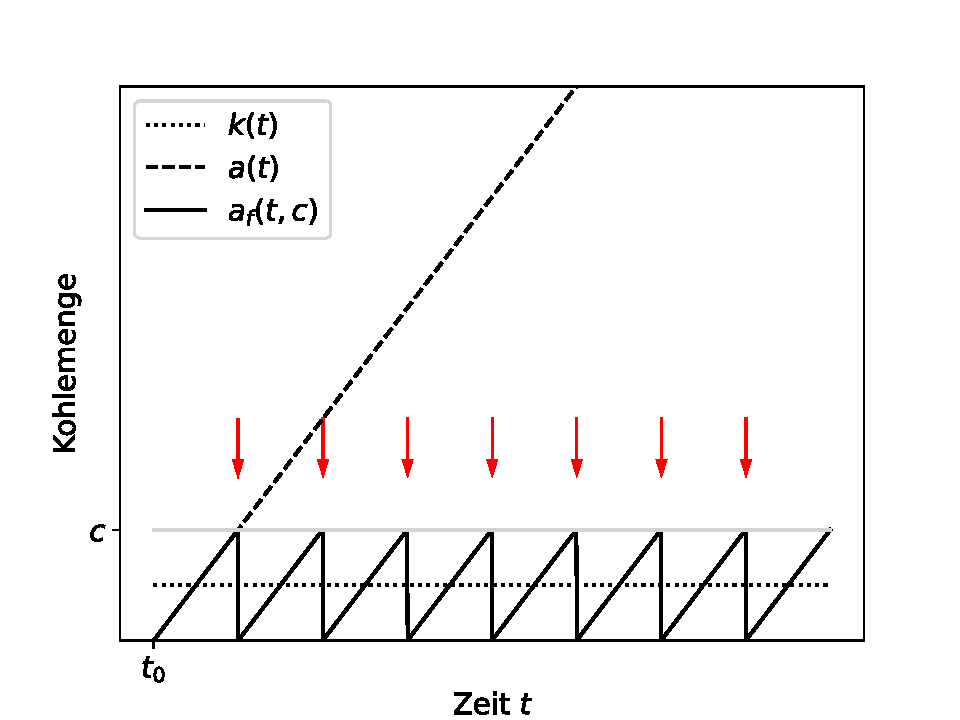
\includegraphics[width=1.0\linewidth]{images/demand-math.pdf}
	\caption{Schematisches Verhalten eines bedarfsorientierten Abfahrtsplans mit dem Kohlebedarf $k(t)$, dem akkumulierten Kohlebedarf $a(t)$ und der akkumulierten Kohlemenge abzüglich der transportierten Kohlemenge $a_{mod}(t,c)$. Die roten Pfeile markieren die Abfahrtszeiten der Kohlezüge.}
	\label{fig:demand-math}
\end{figure}